\section{ATLAS Detector Upgrade}

\subsection{High Luminosity Large Hadron Collider - HL-LHC}
The Large Hadron Collider (LHC), run by CERN at the Franco-Swiss border near Geneva, is a circular accelerator with 27 km of acceleration pipes, is the largest scientific instrument ever designed and built for scientific research. Successfully commissioned in March 2010 for proton-proton collision with a 7 GeV centre-of-mass energy.\\
The LHC is pusshing the limits of human knowledge, enabling physicist to go beyond Standar Model (SM): the enigmatic Higgs boson, mysterious Dark Matter and the world of supersymetry are just three of the long-awaited mysterous that the LHC will unveil. The announcement given by CERN on 4 July 2012 about the discovery of new boson at 125-126 GeV, almost certainly the long awaited Higgs particle, is the first fundamental discovery, hopefully the first of a series, that the LHC can deliver.\\
Such discovery was thanks to the different detectors located on the four interaction points; ALICE, LHCb, CMS and ATLAS. This last one is the detector where our university is taking part.\\
\begin{figure}[ht]
		\centering
		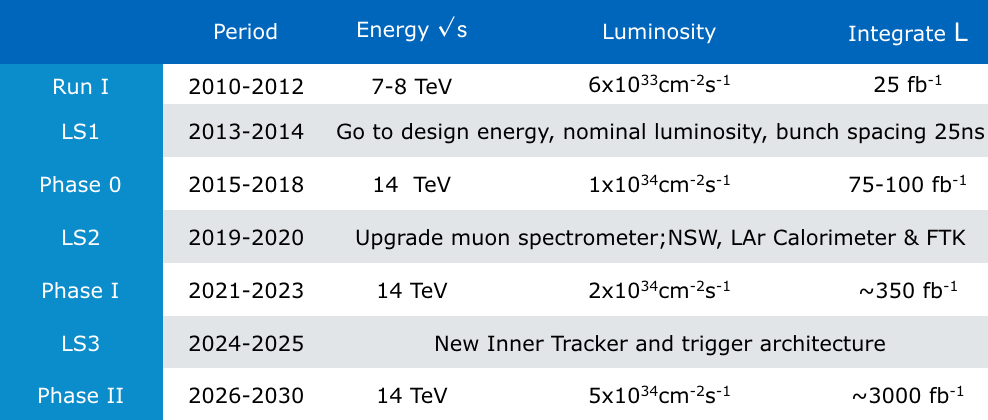
\includegraphics[width=0.7\textwidth]{LHC_program_table.png}
		\caption{LCH Schedule}\label{fig:a}
\end{figure}
\par
CONTINUE WITH LHC UPGRADE and GOALS

\subsection{ATLAS Detector}
The ATLAS detector it is a general-purpose detector, designed to explore proton-proton colissions at center of mass up to $\sqrt{s}=$14 GeV. Looking for.... \par
Such energy has been achived from 2015 and successfuly working with a luminosity of 1x10$^{34}$cm$^{-2}s^{-1}$ from 2016.\\

Describe ATLAS detector and its part, together with the problem faced by now.\par


ENDING WITH THE FAKE TRIGGERS AND PROBLEMS FOR LOW PT.\par 



\subsection{New Small Wheel}

In manner to fullfill the LHC program (in fig.\ref{fig:a}), and in order to benefit from the expected high luminosity performance that will be provided by the
Phase-I upgraded LHC, the first station of ATLAS muon end-cap system (Small Wheel, SW) will need to be replaced.  The New Small Wheel (NSW) will have to operate
in a high background radiation region (upto 15kHz/cm$^2$) while reconstructing muon tracks with high precision as well as furnishing information for the Level-1
trigger. These performance criteria are demanding. In particular, the precision reconstruction of tracks for offline analysis requires a spatial resolution
about 100 $\mu$m, and the Level-1 trigger track segments have to be reconstructed online with an angular resolution of symroximately 1mrad. The NSW will have to
chamber technologies, one primarily devoted to the Level-1 trigger function (small-strip Thin Gap Chambers, sTGC) and one dedicated to precision tracking
(Micromegas detectors, MM). The sTGC are primarily deployed for triggering given their single bunch corssing identification capability. The MM detectors have
exceptional precision tracking capabilities due to their small gap (5mm) and strip pitch (symroximately 0.5mm). Such a precision is crucial to maintain the
current ATLAS muon momentum resolution in the high background environment of the upgraded LHC. The MM chambers can, at the same time, confirm the existence of a
track segments found by the muon end-cap middle station (Big Wheels) online. The sTGC also has the ability to measure offline muon tracks with good precision,
so the sTGC-MM chamber technology combination forms a fully redundant detector system for triggering and tracking both for online and offline functions. This
detector combination has been designed to be ablo to also provide excellente performance for the eventual High Luminosity LHC upgrade.\par 



\section{Small-strip Thing Gap Chamber}

The Small strip Thin Gap Chamber (a.k.a sTGC) detector it is a multi-wire proportional chamber (MWPC)  working in a high gain mode with a cathode-anode pitch smaller than the anode-anode pitch, mostly based on the design of the Thin Gap Chamber\cite{tgc}, with thinner strips as the main improvement from the previous version. The TGC tecnology has been used since 1988 in OPAL experiment and currently are part of the the muon spectrometer in ATLAS. \\
	This new  chamber has the advantage of having a 3.2mm strip width compare to the \textcolor{red}{5-6 mm} from the previous TGC, that is why it is called small strip Thin Gap Chamber.\\ 
	The size of the strips has been choosen to cope up with the precision resolution require for the NSW (explained before), where it has to be better than 100 $\mu$m and provide a reponse with a few nanoseconds. For this purpose, chambers with different strips sizes has been build and test under pion beams, chosed the 3.2mm has the best option\cite{stripwidth}. \par
%-------- sTGC Explanation -------

The sTGC is made of two resistive cathods planes, one with csymer strips and the other with pads, each cathode plane is made of FR4 with 1.6mm of thickness, where  100
$\mu$m of csymer is etched for strips (pads) and then pressed with a 100 $\mu$m of FR4 over it and then sprayed with
graphite to provide 100-200 k$\Omega / \square$ (1 M$\Omega/\square$ for TGC) so it can be treatead as a resistive cathode plane.\\
The anodes are golden tungsten wires of 50 $\mu$m diameter, distributed at 1.8 mm between each other. The gas gap (2.8mm) is filled with a mixture of carbon dioxide (CO$_2$) and n-pentane(C$_5$H$_12$) in proportion 55:45 respectively both
strongly quenching gases that provide a high amplification factor and relatively low sensitivity to mechanical variations.\textcolor{red}{[ref Mechanical
variations]}\\  

%----------- How its produce the ionization and drifts  -----

%----------- sTGC mode picture -----

\begin{figure}[h]
		\centering
		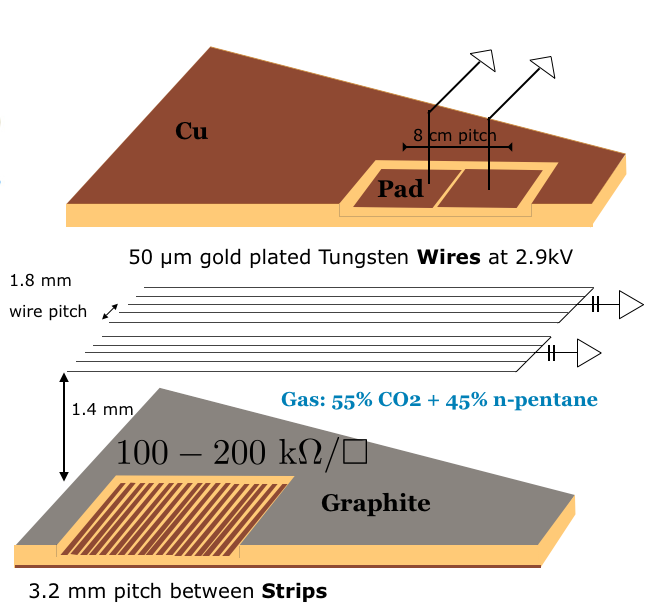
\includegraphics[width=0.5\textwidth]{sTGC_layout.png}
		\caption{Single plane sTGC}\label{fig:sTGC}
\end{figure}

A MWPC detector type  is a relativetely old technology, its succesfuly introduction to detector system in 1968 gave the Nobel prize to George Charpak in 1992. This device has
been a major ingrediente in detector systems since it can achieve spatial resolutions of 500 $\mu$m or less, and has typical time resolution of about 30 ns.\\
The TGC has been built as a MWPC with a thinner gas gap, its means, the distance from the anode-cathode is smaller than the anode-anode (wire to wire) to
provide a fast time response, and at the same time giving a higher amplification, to achieve this smaller distance, precautions must be taken into account when
the internal pieces are construct, for that a precision of 50 $\mu$m must be achieve.\\ To work with such geometry several test were made to find the proper gas
mixture\cite{gaschoice}. Find the most suitiable mixture of  55\% well known carbon dioxide as a quenching gas, and a 45\% of n-pentane, which for his nature
can absorb energy in many ways of molecules  degree of freedom, vibrational, rotational, etc.\\ 


\begin{itemize}
\item voltaje de operacion.
\item resitividad del graphito y para que usamos grafito.
\item Que es lo moderno de este detector...
\end{itemize}


\section{Construction process}
Cathode production and how we achieve the resolution requeride for this.\\
Clean cathode\\
Sprayed process\\
Achieve the proper superficial resistivity\\
glue internal parts\\
Winding wires, soldered and clean afterwards\\
test wires under hv\\
Close chamber and filled with CO$_2$, no sparks must found\\
glue chamber\\
Thickness measurments\\
Repeat process till get 4 modules\\
Overall thickness measurements and pin position check\\


\section{Gain uniformity measurements}

After the chambers are built it is important to know the response of the detector, es and a primivite way to do such thing without any electronic readout attach
to strips or wires, is to measure the current draw from the power ssymly and see how it behaves to a radiation source.\\ There are two ingredients that can
produce gain variations on wire detectors, the first one is the "nature" gain fluctuations from the charge production in proportional counters which follow
Polya distribution, however is less pronounced in semi-proportional mode such as sTGC working region.\\ The second one is related to the mechanical tolerances,
this part is very well known since 40 years as it is presented on Sauli book about drift chambers and tell us that for a diameter variations of the wire about
1\% (fabrication precision) will result on a 3\% change in the gain, where as about \unit{100}{$\mu$ m} difference in the gas gap thickness (\unit{2.7}{mm})
results in about 15\% chage of the gain. the effecto of a wire displacment of about \unit{100}{$\mu$ m} of a wire plane results in 1\% int the charge of the two
adjacent wires which with a gain of $\sim 10^6$ will give a $\sim 10\%$ change in the gain.\\ Taking all of this in consideration is expected to get a gain variation less
than 20\% as Quality Acceptance.\\ In this test the gain is considered as the current draw measured from the power ssymly and its need to test under two
different working points (bias voltage), one when the chamber it is not in the limited proportional region, 2500 volts, a take it as a reference compare to the
2900 volts which is the operational voltage.\\

%-------- why x ray source ? ----------

For such test the x-ray source is used due to the many advantages;

\begin{itemize}
	\item Mostly monoenergetic photons.
	\item Variable current: which can provides diferent rates. [\unit{1}{$\mu$A} - \unit{200}{$\mu$A}]
	\item Variable voltage: modifyng breaking voltage of electrons inside the x-ray gun. [\unit{10}{keV} - \unit{50}{keV}]
	\item Different spot size: with a set of collimator it is posible to irradiate only interesting area.
	\item Portable, it is possible to move accross the sensitive area of the detector.
\end{itemize}

\subsection{Setup}
Provide explanation of setup and posterior details of instruments.\\

\begin{itemize}
\item X-ray source: Mini-X gun with photons of  50 keV and flux of  45 $\mu$A
\item Collimator: 5º.
\item Distance from source: 2.5 $\pm$ 0.3 cm. Spot size: 2 $\pm$ 0.26 mm.
\item KUKA arm; giving vertical steps:1.5 cm, horizontal steps: 5 cm.
\item HV power ssymly: 50 nA resolution. Sampling rate: 1 sample/s.
\end{itemize}


\subsection{Results}

\begin{figure}[ht]
	\centering
	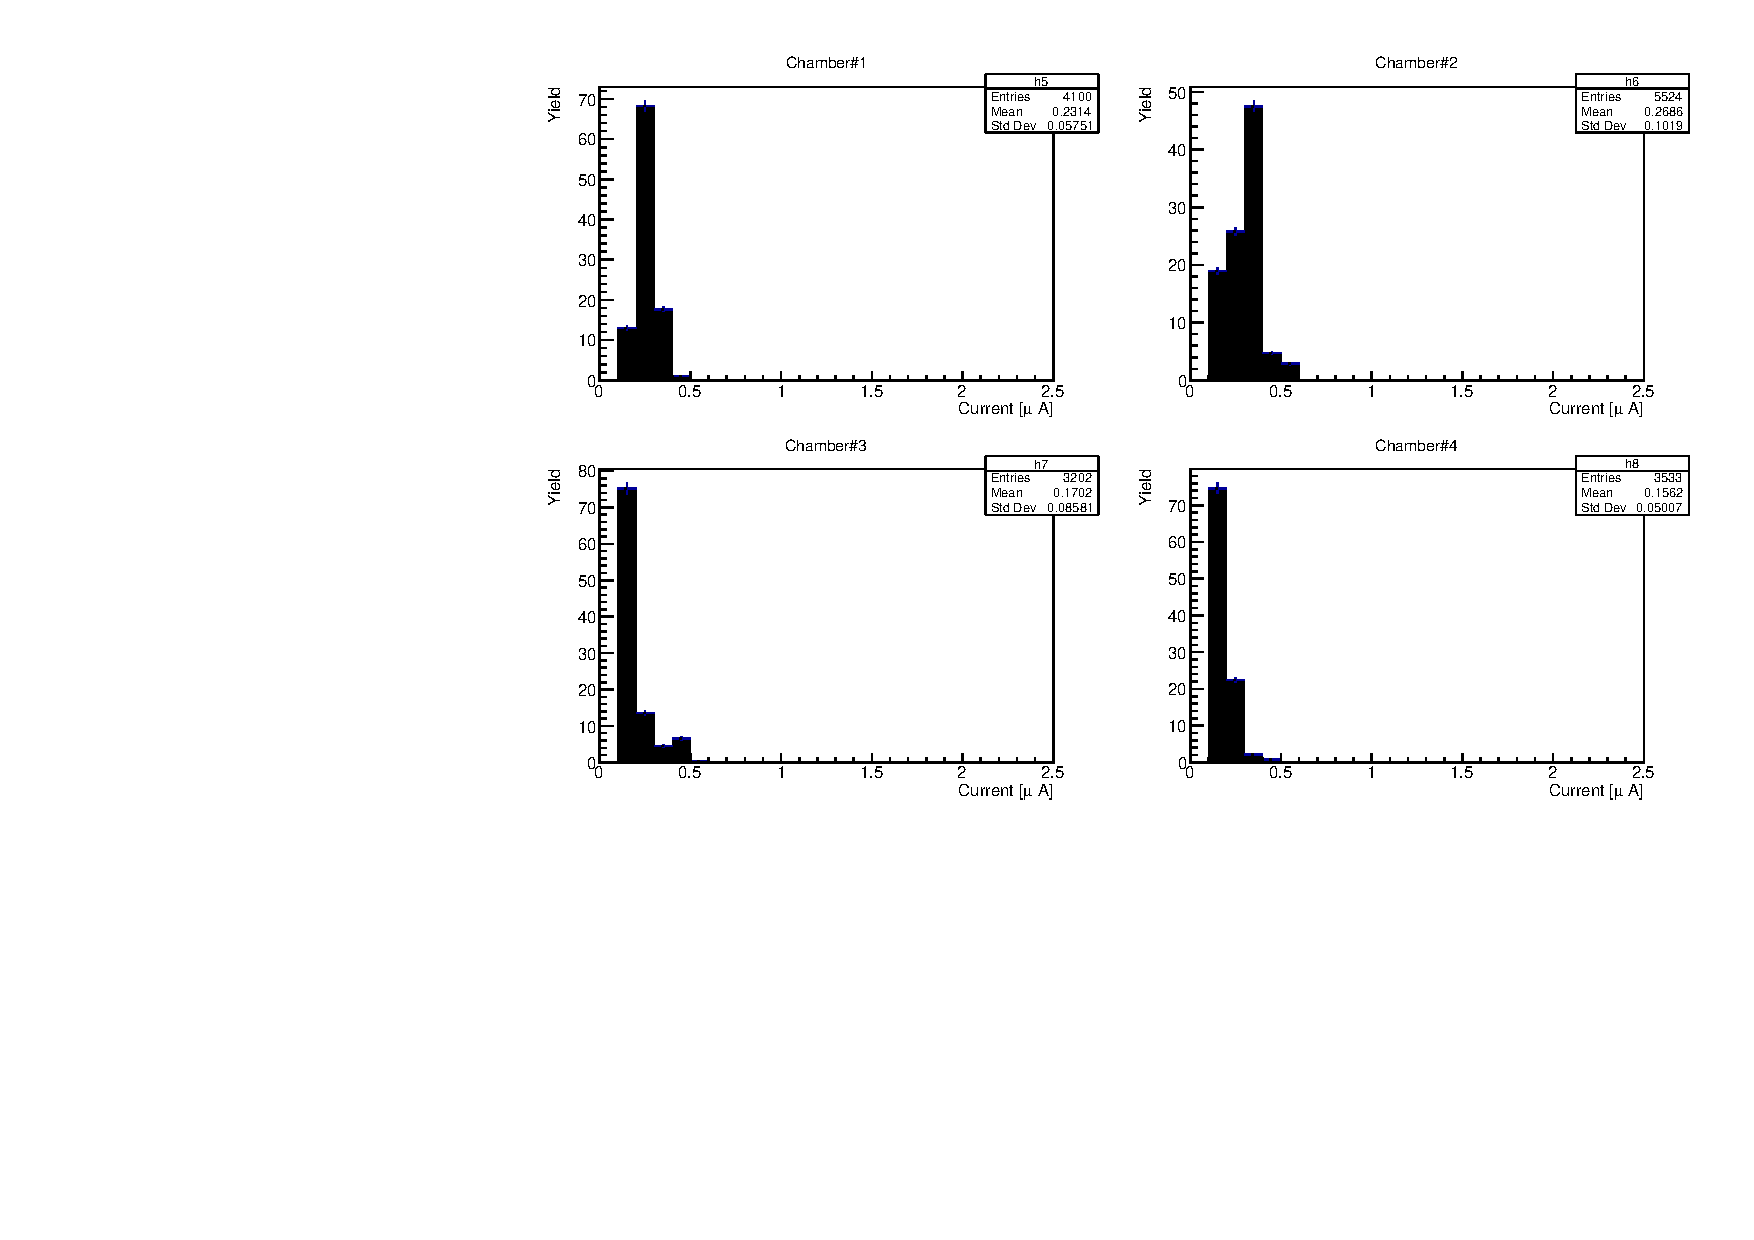
\includegraphics[width=0.7\textwidth]{uniformity_2500.pdf}
	\caption{Current draw from power ssymly at 2500V}\label{fig:2500V}
\end{figure}

\begin{figure}[hb]
	\centering
	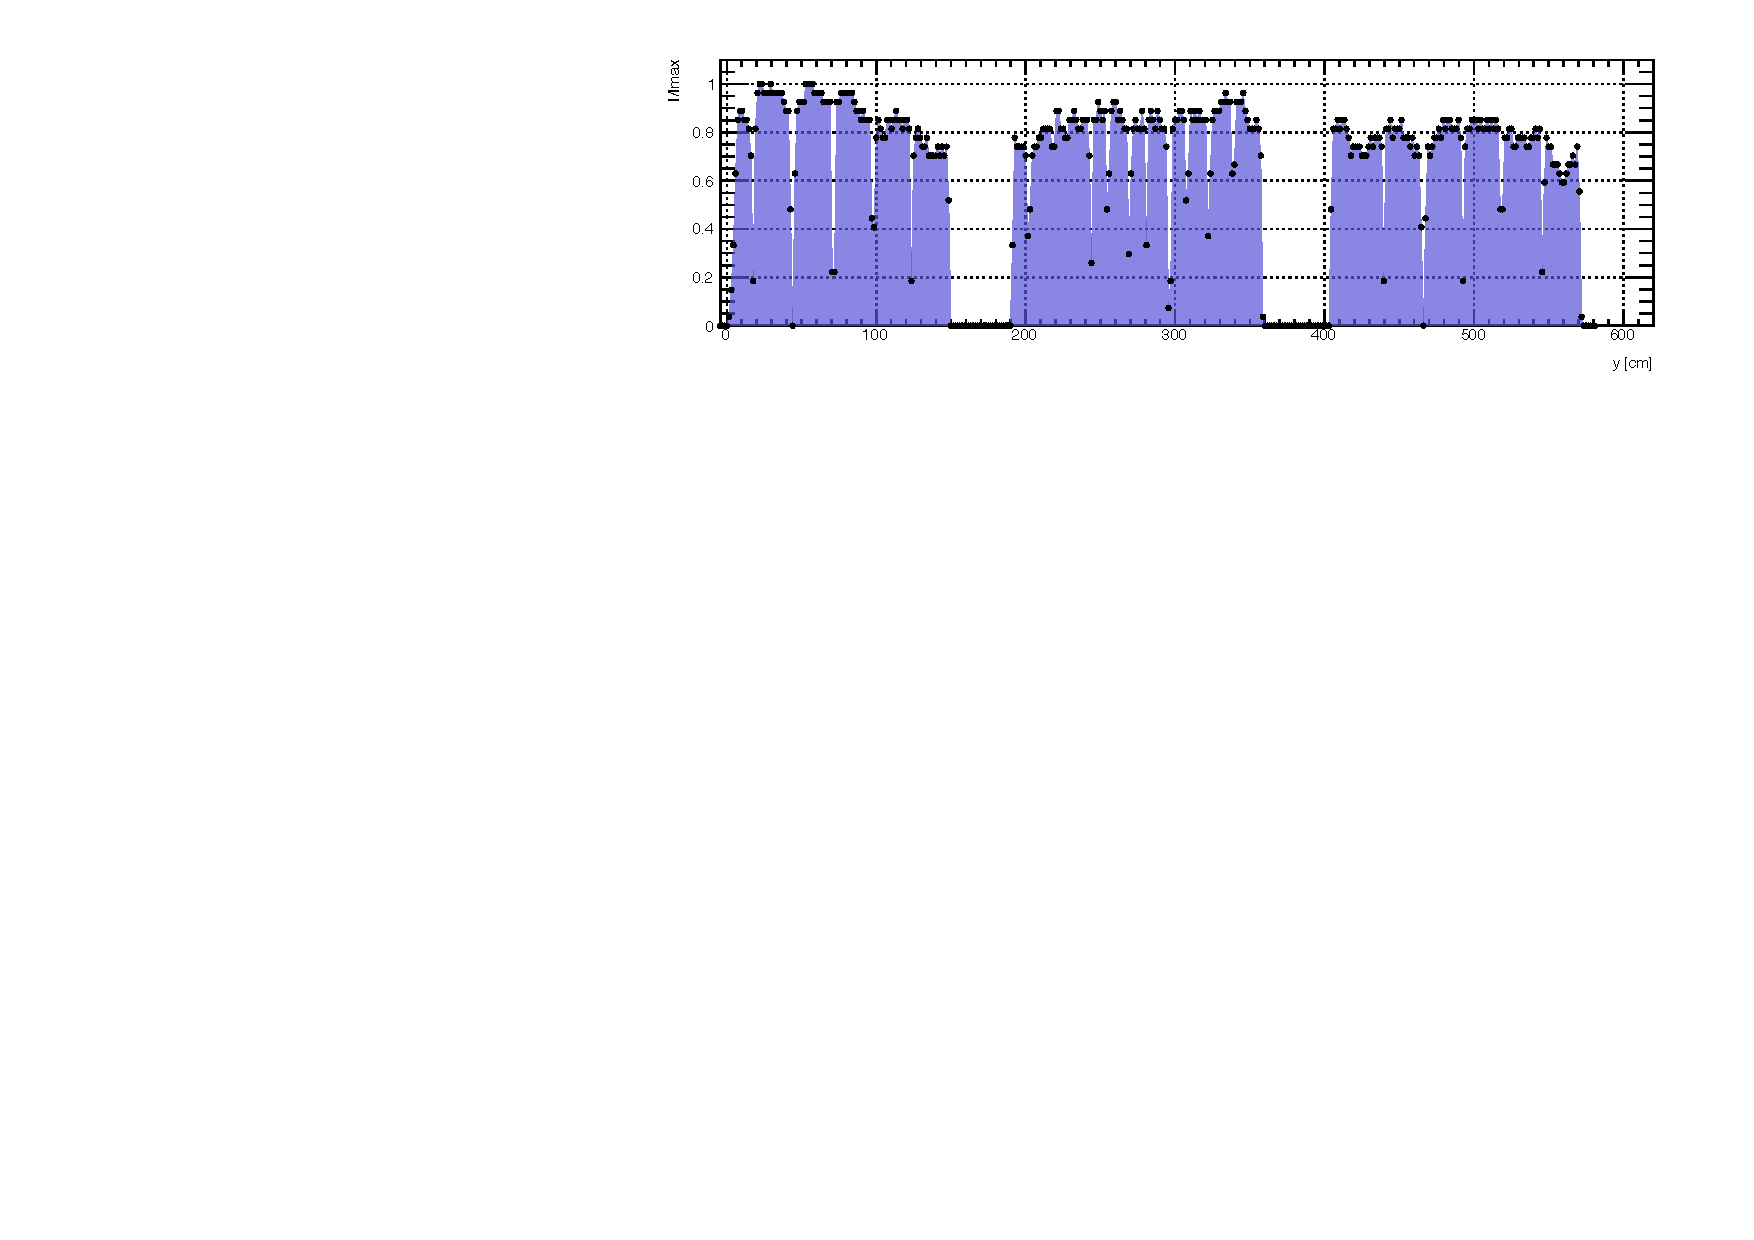
\includegraphics[width=0.7\textwidth]{uniformity_2900.pdf}
	\caption{Current draw from power ssymly at 2900V}\label{fig:2900V}
\end{figure}


\section{Test under high rate}


\section{Spatial resolution strips}

\section{Charge sharing between pads}

\section{summary}
